\subsection{Input features} \label{inputfeatures}

    \subsubsection{Global features}

        \paragraph{Protein length}

      	    Protein length is computed as the number of residues in the protein sequence.
    	    It provides complementary information that convolutional layers cannot capture.
     	    Indeed, fully-connected neural networks have the ability to handle arbitrary-sized
    	    features maps at the cost of not knowing the dimensionality of their inputs.
    	    Injecting protein length as a supplementary global feature may help the model
    	    to infer the maximum distance in long-range contacts.

	   \paragraph{Effective number of sequences} \label{meff}

    	    The number of effective sequences is equal, w.r.t. to a given threshold,
    	    to the number of non-redundant sequences in the set of homologous sequences.
    	    It provides a bound on the potential performance of the DCA methods involved
    	    in the pipeline.

            \begin{equation}
                M_{eff} = \sum_{i=1}^m w_i = \sum_{i=1}^m \frac{1}{|\{r(s_i, s_j) \ge \tau \quad \forall j \in \{1, \dotsc, m\}\}|}
            \end{equation}

            $w_i$ is the weight associated to homologous sequence $i$.
            $r(s_i, s_j)$ is the identity rate between sequences $s_i$ and $s_j$, in other words
            the number of matching residues (including gaps) divided by the total number of positions,
            which is assumed to be equal in both sequences.

    \subsubsection{1-dimensional features}

        \paragraph{One-hot encoded sequence}

            Given an amino acid sequence $\{s_1, s_2, \ldots,
            s_L\}$ of size L, the one-hot encoded sequence
            is a matrix $X \in \{0, 1\}^{L \times 21}$
            where $x_{ia}$ is one if $s_i = a$ and zero otherwise.

        \paragraph{Solvent accessibility prediction}

            Solvent accessibility or solvent-accessible surface is the surface of
            a molecule that is accessible to a solvent. Such feature contains indirect
            information about the protein structure since residues with low accessibility
            are more likely to be internal to the protein and vice versa.
            When atomic coordinates are available, solvent accessibility can be computed exactly
            using the rolling ball algorithm from Shrake and Rupley~\cite{shrake1973environment},
            as illustrated by figure~\ref{rollingball}.
            Since protein structure is not available for target proteins of the test set,
            supervised models rely on predicted solvent accessibility instead.

            \begin{figure}[H]
                \begin{center}
                    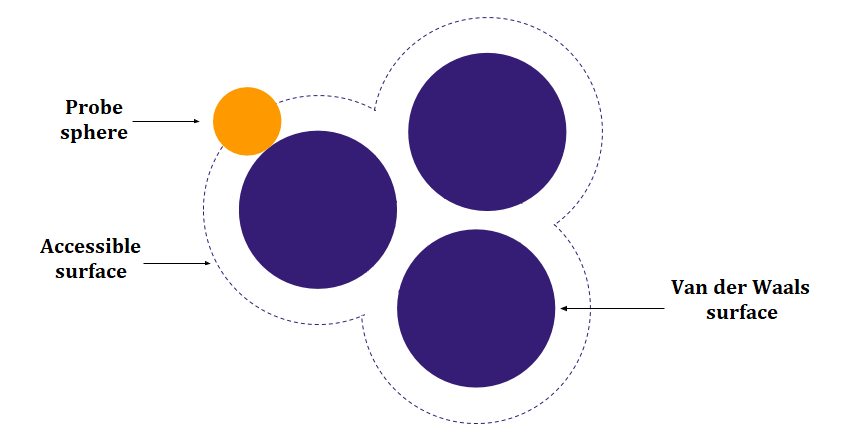
\includegraphics[height=5cm, keepaspectratio]{imgs/accessibility.png}
                    \caption{Accessible surface, obtained by "rolling" a probe sphere (a molecule
                        of solvent, colored in orange) on the Van der Waals surface of a biomolecule
                        (colored in blue).}
                    \label{rollingball}
                \end{center}
            \end{figure}

            The RaptorX-Property server~\cite{wang2016raptorx} is publicly available and provides
            predictions for relative solvent accessibility (RSA). The latter is defined as the predicted
            accessible surface of a residue divided by the maximum possible solvent accessibility
            for that amino acid, which is more convenient more machine learning since it does not a
            normalization step. RSA prediction is 3-state. A residue can be either:
            \begin{itemize}
                \item Buried (B), when RSA is below 10\%.
                \item Intermediate (I), when RSA is between 10\% and 40\%.
                \item Exposed (E), when RSA is above 40\%.
            \end{itemize}


        \paragraph{Predicted secondary structure prediction}

            As defined by DSSP, there are 8 different states for encoding
            secondary structure: H (alpha-helix),
            G (310 helix), I (pi-helix), E (beta-strand), B (beta-bridge),
            T (beta-turn), S (high curvature loop) and L (irregular loop).
            In practice, secondary structure prediction is either 3-state
            or 8-state~\cite{wang2016raptorx}.
            The eight states are: Alpha-helix, 310 helix, Pi-helix, Beta-strand,
            Beta-bridge, Beta-turn, High curvature loop, Irregular loop.

            When the number of labels is limited to three,
            the predictor only focuses on beta-strands (E), alpha-helices (H)
            and a third state which is the union of the six remaining states (C).
            Formally, a $m$-state secondary structure prediction is a matrix
            $S \in [0, 1]^{L \times m}$ where element $S_{i,j}$ is the probability
            of residue $i$ being in conformation $j$,
            with each row summing to one.

        \paragraph{Region disorder prediction}

            Region disorder prediction is a vector $D \in [0, 1]^L$
            where $D_i$ is the probability of residue $i$ being in a region
            of missing residues in the X-ray 3D structure. Residues with high
            probability are said to be disordered.
            Such features are also made publicly available by the 
            RaptorX-Property server~\cite{wang2016raptorx}.

        \paragraph{Amino acid frequencies}

            Amino acid frequencies are position-specific features that can be efficiently computed.
            Let $S \in \{0, \ldots, \naatypes\}^{M \times L}$ be a
            Multiple sequence alignment matrix containing $M$ sequences aligned to a target
            sequence of length $L$. Then amino acid frequencies can be arranged
            in a matrix $F \in \mathbb{R}^{L \times \naatypes}$
            where element $F_{ia}$ is computed as follows:

            \begin{equation}
                F_{ia} = \frac{1}{M} \sum\limits_{k=1}^M \delta(S_{ki}, a)
            \end{equation}

        \paragraph{Position-Specific Scoring Matrix}

            The position-specific scoring matrix~\cite{jones1999protein} is 
            computed on the whole multiple sequence alignment as well.
            It is of shape $F \in \mathbb{R}^{L \times \naatypes}$ like the amino acid frequency matrix
            but is more informative as it summarizes common patterns present in the alignment.

        \paragraph{Atchley factors}

            Atchley factors are residue-specific constant values resulting from the factor analysis
            of Atchley~\cite{Atchley2005}. There are 5 factors:
            \begin{itemize}
                \item Factor I is a polarity index but incorporates many variables like polarity, hydrophobicity,
                    the covariance of the proportion of exposed residues (with low surface accessibility), the
                    number of hydrogen bond donors, etc.
                \item Factor II is a secondary structure factor that is inversely related to the propensity of the
                    amino acid to be in a specific structural state.
                \item Factor III is related to the residue size: residue volume, average volume when buried, residue weight, etc.
                \item Factor IV is related to the amino acid composition: number of codons, etc.
                \item Factor V is an electrostatic charge index.
            \end{itemize}

        \paragraph{Self-information}

            In information theory, self-information is the amount of information, in bits,
            obtained by observing a random variable. In particular, let $x_{ij} \in \{0, 1\}$ be
            a binary variable indicating the presence of an amino acid of type $j$ at site $i$.
            The self-information suggested by Michel et al~\cite{Michel383133} can be formalized
            with the following equation:

            \begin{equation}
                I_{ij} = \log_2 (p_{ij} / \langle p_i \rangle)
            \end{equation}

            where $p_{ij}$ is the probability of observing amino acid $j$ at site $i$ among all residues
            of given MSA, and $\langle p_j \rangle$ is the frequency of amino acid $j$
            in the Uniref50 dataset.

        \paragraph{Partial entropies}

            \todo{ \cite{Michel383133}}

            \begin{equation}
                S_i = p_i \log_2 (p_i / \langle p_i \rangle)
            \end{equation}

    \subsubsection{2-dimensional features}

        \paragraph{Mutual Information and Normalized Mutual Information}

            Following the formalism described in \cite{Michel383133}, MI is described as:

            \begin{equation}
                MI(x, y) = \sum\limits_{x, y} P(x, y) \log \Big( \frac{P(x, y)}{P(x) \cdot P(y)} \Big)
            \end{equation}

            \begin{equation}
                NMI(x, y) = \frac{MI(x, y)}{\sqrt{S(x) \cdot S(y)}}
            \end{equation}

            Average product correction is applied to both MI and NMI.

        \paragraph{Cross-entropy}

            Cross-entropy is computed in \cite{Michel383133} using the following formula:

            \begin{equation}
                H(x, y) = S(x) + S(y) - MI(x, y)
            \end{equation}

        \paragraph{Contact potential}

            \todo{}

        \paragraph{Evolutionary couplings}

            Predictions from GaussDCA, plmDCA or PSICOV are the most discriminative features
            used in supervised methods. Only top predicted contacts are informative, but deep
            architectures help refining predicted couplings into high-quality contact maps.

        \paragraph{Covariance}

            Covariance matrices are computed as in equation \ref{covariance} from the section
            about Gaussian graphical models (see section \ref{graphicalmodels}).
            In PSICOV~\cite{doi:10.1093/bioinformatics/btr638}, the inferred covariance
            matrix is averaged across the dimension of amino acid types.
            In DeepCov~\cite{doi:10.1093/bioinformatics/bty341}, the full matrix is used
            as input to the supervised model.

    \subsection{Features for the proposed approach}

        The lines which will follow are a discussion about the features to use as inputs
        to the model. At the outset, it should be noted that all models rely on
        two-dimensional features. Those features are either predictions from another
        predictor, covariance matrices or correlated mutations.
        However, using intermediary predictions requires installing additional software.
        PSICOV is written in C and can be recompiled. The official implementation of
        plmDCA was originally made in Matlab, forcing researchers to add a whole raft
        of external tools. plmDCA, as well as GaussDCA now have a Julia implementation,
        making them more accessible. The proposed approach incorporates all three
        predictors in its pipeline.

        \begin{landscape}
            \begin{table}[H]
                \centering
                \begin{tabular}{llcccccc}
                    \hline
                    Features & & DeepCov & DeepContact & PConsC4 & DNCON2 & RaptorX & Proposed method \\
                    \hline
                    \hline
                    Global & Protein length & & & & $\times$ & & $\times$ \\
                    & Meff & & & & $\times$ & & $\times$ \\
                    \hline
                    1-dimensional & Column log-entropy & & $\times$ & & & & \\
                    & Predictors stdv & & $\times$ & & & & \\
                    & Encoded sequence & & & $\times$ & & & $\times$ \\
                    & \textbf{Solvent accessibility} & & $\times$ & & $\times$ & $\times$ & $\times$ \\
                    & \textbf{Predicted SS} & & $\times$ & & $\times$ & $\times$ & $\times$ \\
                    & AA frequencies & & $\times$ & $\times$ & & & \\
                    & PSSM & & & & $\times$ & $\times$ & \\
                    & Atchley factors & & & & $\times$ & & \\
                    & Self-information & & & $\times$ & & & $\times$ \\
                    & Partial entropies & & & $\times$ & & & $\times$ \\
                    \hline
                    2-dimensional & Mutual Information (MI) & & & $\times$ & $\times$ & $\times$ & $\times$ \\
                    & Normalized MI & & $\times$ & $\times$ & $\times$ & & $\times$ \\
                    & Cross-entropy & & $\times$ & $\times$ & & & $\times$ \\
                    & \textbf{Contact potential} & & & & & $\times$ & \\
                    & \textbf{EVFold} & & $\times$ & & & & \\
                    & \textbf{CCMPred} & & $\times$ & & $\times$ & $\times$ & \\
                    & \textbf{plmDCA} & & & & $\times$ & & \\
                    & \textbf{GaussDCA} & & & $\times$ & & & $\times$ \\
                    & \textbf{PSICOV} & & & & & & \\
                    & Covariance & $\times$ & & & & & \\
                    \hline
                \end{tabular}
                    \caption{Features used in state-of-the-art deep learning approaches.
                        Feature extraction methods that rely on external tools (excluding
                        MSA tools) are highlighted in bold.}
                    \label{features}
            \end{table}
        \end{landscape}
